%% ============================================================
%% Paper01_ChildSponsorship.tex
%% International child sponsorship impact on the intended choice
%% of acquiring a higher education degree: the case of rural Mexico
%% Daniel Prudencio -- Education Economics (2025)
%%
%% Compile: cd Slides
%%   TEXINPUTS=../Preambles:$TEXINPUTS xelatex -interaction=nonstopmode Paper01_ChildSponsorship.tex
%%   BIBINPUTS=..:$BIBINPUTS bibtex Paper01_ChildSponsorship
%%   TEXINPUTS=../Preambles:$TEXINPUTS xelatex -interaction=nonstopmode Paper01_ChildSponsorship.tex
%%   TEXINPUTS=../Preambles:$TEXINPUTS xelatex -interaction=nonstopmode Paper01_ChildSponsorship.tex
%% ============================================================
\documentclass[aspectratio=169, 10pt]{beamer}
%% ============================================================
%% header.tex -- Shared Beamer preamble for Research Portfolio
%% Compile with: XeLaTeX (3-pass + bibtex)
%% Colors match Quarto/emory-clean.scss for cross-format consistency
%% ============================================================

%% ---- Packages -----------------------------------------------
\usepackage{fontspec}           % XeLaTeX font loading
\usepackage{unicode-math}       % Unicode math support
\usepackage{amsmath, mathtools} % Math environments
\usepackage{booktabs}           % Publication-quality tables
\usepackage{multirow}           % Multi-row table cells
\usepackage{graphicx}           % Include figures
\usepackage{xcolor}             % Color definitions
\usepackage{tcolorbox}          % Colored boxes
\tcbuselibrary{skins, breakable}
\usepackage{natbib}             % Author-year citations
\usepackage{appendixnumberbeamer} % Appendix slides don't count in total
\usepackage{hyperref}           % Hyperlinks
\usepackage{tikz}               % Diagrams (if needed)

%% ---- Fonts --------------------------------------------------
%% Using TeX Gyre Heros (Helvetica-style, bundled with MiKTeX).
%% To switch to Source Sans Pro: install it, then swap the two blocks below.
\setmainfont{TeX Gyre Heros}
\setsansfont{TeX Gyre Heros}
% Alternative: uncomment below and comment above if Source Sans Pro is installed
% \setmainfont{Source Sans Pro}[BoldFont=Source Sans Pro SemiBold]
% \setsansfont{Source Sans Pro}[BoldFont=Source Sans Pro SemiBold]

%% ---- Colors (matching emory-clean.scss) ---------------------
\definecolor{navyblue}{HTML}{012169}
\definecolor{institutgold}{HTML}{2E75B6}   % steel blue (was gold #B9975B)
\definecolor{highlightyellow}{HTML}{F2A900}
\definecolor{lightbg}{HTML}{E8EDF5}
\definecolor{darkgray}{HTML}{1a1a1a}
\definecolor{medgray}{HTML}{555555}
\definecolor{lightgray}{HTML}{f8f9fa}
\definecolor{positivegreen}{HTML}{15803d}
\definecolor{negativered}{HTML}{b91c1c}

%% ---- Beamer Theme -------------------------------------------
\usetheme{default}
\usecolortheme{default}
\setbeamertemplate{navigation symbols}{}   % No navigation clutter

%% Frame title
\setbeamercolor{frametitle}{fg=white, bg=navyblue}
\setbeamertemplate{frametitle}{%
  \vspace*{0.3em}%
  \insertframetitle%
  \vspace*{0.3em}%
}
\setbeamerfont{frametitle}{series=\bfseries, size=\large}

%% Title page colors
\setbeamercolor{title}{fg=navyblue}
\setbeamercolor{subtitle}{fg=institutgold}
\setbeamercolor{author}{fg=navyblue}
\setbeamercolor{institute}{fg=medgray}
\setbeamercolor{date}{fg=institutgold}

%% Body
\setbeamercolor{background canvas}{bg=white}
\setbeamercolor{normal text}{fg=darkgray}
\setbeamerfont{normal text}{family=\sffamily}

%% Itemize bullets
\setbeamercolor{item}{fg=navyblue}
\setbeamercolor{subitem}{fg=institutgold}
\setbeamertemplate{itemize item}{\small\textbullet}
\setbeamertemplate{itemize subitem}{\small$\rightarrow$}

%% Block environments
\setbeamercolor{block title}{fg=white, bg=navyblue}
\setbeamercolor{block body}{fg=darkgray, bg=lightbg}
\setbeamercolor{block title alerted}{fg=white, bg=institutgold}
\setbeamercolor{block body alerted}{fg=darkgray, bg=white}

%% Footer
\setbeamertemplate{footline}{%
  \hfill%
  \usebeamerfont{page number in head/foot}%
  \usebeamercolor[fg]{page number in head/foot}%
  \insertframenumber\,/\,\inserttotalframenumber\kern1em%
  \vskip4pt%
}
\setbeamercolor{page number in head/foot}{fg=medgray}

%% Section slides (automatically centered, navy bg)
\AtBeginSection[]{%
  \begin{frame}[plain]
    \begin{tikzpicture}[remember picture, overlay]
      \fill[navyblue] (current page.south west) rectangle (current page.north east);
      \node[white, font=\bfseries\Large, align=center] at (current page.center)
        {\insertsectionhead};
    \end{tikzpicture}
  \end{frame}%
}

%% ---- Custom Box Environments --------------------------------

%% keybox: gold background, for key takeaways
\newtcolorbox{keybox}{%
  colback=institutgold!12!white,
  colframe=institutgold,
  leftrule=4pt, rightrule=0pt, toprule=0pt, bottomrule=0pt,
  arc=4pt, outer arc=4pt,
  boxsep=2pt, left=6pt, right=6pt, top=5pt, bottom=5pt,
}

%% methodbox: navy left bar, for model/identification
\newtcolorbox{methodbox}{%
  colback=navyblue!5!white,
  colframe=navyblue,
  leftrule=4pt, rightrule=0pt, toprule=0pt, bottomrule=0pt,
  arc=4pt, outer arc=4pt,
  boxsep=2pt, left=6pt, right=6pt, top=5pt, bottom=5pt,
}

%% resultbox: gold border, for main findings
\newtcolorbox{resultbox}{%
  colback=institutgold!10!white,
  colframe=institutgold,
  leftrule=2pt, rightrule=2pt, toprule=2pt, bottomrule=2pt,
  arc=4pt, outer arc=4pt,
  boxsep=2pt, left=6pt, right=6pt, top=5pt, bottom=5pt,
}

%% assumptionbox: titled, formal assumptions
\newtcolorbox{assumptionbox}[1][]{%
  colback=highlightyellow!8!white,
  colframe=highlightyellow!70!black,
  leftrule=2pt, rightrule=2pt, toprule=2pt, bottomrule=2pt,
  arc=4pt, outer arc=4pt,
  boxsep=2pt, left=6pt, right=6pt, top=5pt, bottom=5pt,
  title={#1},
  fonttitle=\bfseries\small,
  attach boxed title to top left={yshift=-2mm, xshift=6pt},
  boxed title style={colback=highlightyellow!70!black, arc=2pt},
}

%% ---- Convenience Commands -----------------------------------
\newcommand{\gold}[1]{{\color{institutgold}\textbf{#1}}}
\newcommand{\navy}[1]{{\color{navyblue}\textbf{#1}}}
\newcommand{\pos}[1]{{\color{positivegreen}\textbf{#1}}}
\newcommand{\bad}[1]{{\color{negativered}\textbf{#1}}}   % red annotation
\newcommand{\hi}[1]{{\color{navyblue}\textbf{#1}}}
% Note: \alert is Beamer built-in (styled gold via alerted text color below)
\setbeamercolor{alerted text}{fg=institutgold}

%% ---- Math shortcuts -----------------------------------------
\newcommand{\E}{\mathbb{E}}
\newcommand{\Prob}{\mathbb{P}}
\newcommand{\ATE}{\mathrm{ATE}}
\newcommand{\ATT}{\mathrm{ATT}}
\newcommand{\MTE}{\mathrm{MTE}}
\newcommand{\Norm}{\mathcal{N}}


%% ---- Bibliography -------------------------------------------
\bibliographystyle{aer}
\setcitestyle{authoryear, open={(}, close={)}}

%% ============================================================
\begin{document}

%% ---- 1. Title Slide -----------------------------------------
\begin{frame}[plain]
  \vspace{1.5em}
  \begin{center}
    {\color{navyblue}\Large\bfseries
      International Child Sponsorship Impact on the Intended\\[0.3em]
      Choice of Acquiring a Higher Education Degree:\\[0.3em]
      The Case of Rural Mexico}\\[1em]
    {\color{institutgold}\large\itshape Education Economics (2025)}\\[1.5em]
    {\color{navyblue}\normalsize\bfseries Daniel Prudencio}\\[0.3em]
    {\color{medgray}\small M Csapek SA \,/\, Tecnológico de Monterrey}\\[1.5em]
    {\color{institutgold}\small Published online: 17 May 2025}
  \end{center}
\end{frame}

%% ============================================================
\section{Motivation}
%% ============================================================

%% ---- 2. Big Picture -----------------------------------------
\begin{frame}{Why Study Educational Aspirations in Rural Latin America?}
  \begin{columns}
    \begin{column}{0.55\textwidth}
      \textbf{The puzzle:} Returns to education are positive and significant — yet \gold{educational attainment remains very low}
      \begin{itemize}
        \item Average years of schooling for adults $>$24 in Oaxaca and Chiapas: \textbf{7.5 and 7.2 years} (barely above primary)
        \item Significant returns to higher education exist even for rural populations
      \end{itemize}
      \vspace{0.5em}
      \textbf{Standard explanation:} \bad{external constraints}
      \begin{itemize}
        \item Income, distance to schools, poor health
      \end{itemize}
      \vspace{0.5em}
      \begin{keybox}
        Growing evidence: \gold{internal constraints} — aspirations, grit, self-efficacy, self-esteem — also play a critical role \citep{Cunha2009, Dalton2016, Heckman2012}
      \end{keybox}
    \end{column}
    \begin{column}{0.40\textwidth}
      \begin{methodbox}
        \small
        \textbf{This paper:} Can a holistic child sponsorship program shift children's aspirations toward higher education?
      \end{methodbox}
    \end{column}
  \end{columns}
\end{frame}

%% ---- 3. Compassion International ----------------------------
\begin{frame}{Compassion International (CI): A Holistic Sponsorship Program}
  \begin{columns}
    \begin{column}{0.50\textwidth}
      \textbf{Compassion International:} Third largest child sponsorship program worldwide
      \begin{itemize}
        \item Sponsors $\approx$\textbf{2.2 million children} across \textbf{29 countries}
        \item Faith-based NGO; collaborates with local churches
        \item In Mexico: \textbf{33,360 children} in $>$185 centers
      \end{itemize}
      \vspace{0.5em}
      \textbf{Duration:} Average \textbf{9.3 years} of sponsorship ($\approx$4,000 hrs of organized activities)
    \end{column}
    \begin{column}{0.46\textwidth}
      \textbf{Program components:}
      \begin{itemize}
        \item \gold{In-kind income transfers}: school supplies, uniforms, healthcare
        \item \gold{After-school program}: 5--6 hrs/week (socio-emotional development, academic tutoring)
        \item \gold{Letter exchanges} with sponsor: broadens career horizons
        \item Catastrophic health insurance; access to nurses and doctors
      \end{itemize}
    \end{column}
  \end{columns}
  \vspace{0.5em}
  \begin{keybox}
    Hypothesis: By broadening horizons and alleviating income constraints, CI may raise children's aspirations to pursue further education
  \end{keybox}
\end{frame}

%% ---- 4. Research Question & Contribution --------------------
\begin{frame}{Research Question and Contributions}
  \begin{block}{Research Question}
    Does Compassion International's sponsorship program raise the aspiration of rural Mexican children (ages 12--15) to acquire a higher education degree?
  \end{block}
  \vspace{0.8em}
  \textbf{Three contributions to the CI literature:}
  \begin{enumerate}
    \item \navy{Selection into CI modeled explicitly} using a binary Roy-type model \citep{Aakvik2005} — allows ATE, ATT, and MTE estimation while correcting for non-random selection
    \item \navy{Subjective income expectations} collected and used to estimate perceived returns to education — tests whether beliefs drive aspirations
    \item \navy{Developing-country context:} prior CI studies focus on adult outcomes; this paper focuses on children's aspirations in an early-development setting
  \end{enumerate}
\end{frame}

%% ---- 5. Roadmap ---------------------------------------------
\begin{frame}{Roadmap}
  \tableofcontents
\end{frame}

%% ============================================================
\section{Institutional Framework \& Data}
%% ============================================================

%% ---- 6. CI Program Components (deeper) ----------------------
\begin{frame}{CI's Program: Holistic Development}
  \begin{columns}
    \begin{column}{0.48\textwidth}
      \textbf{Material support:}
      \begin{itemize}
        \item School supplies and uniforms
        \item Food and basic goods
        \item Catastrophic health insurance
        \item Access to affiliated nurses and doctors
      \end{itemize}
      \vspace{0.6em}
      \textbf{Educational support:}
      \begin{itemize}
        \item Academic tutoring (in after-school program)
        \item Spiritual and values-based education
      \end{itemize}
    \end{column}
    \begin{column}{0.48\textwidth}
      \textbf{Socio-emotional development:}
      \begin{itemize}
        \item Classes emphasizing self-efficacy, self-esteem, social trust
        \item Structured extracurricular activities
        \item Letter exchanges with international sponsors
      \end{itemize}
      \vspace{0.4em}
      \begin{methodbox}
        \small The holistic design is the key mechanism: not just income relief but also expanding \gold{perceived career possibilities} and \gold{social horizons}
      \end{methodbox}
    \end{column}
  \end{columns}
\end{frame}

%% ---- 7. CI Selection Process --------------------------------
\begin{frame}{CI's Selection of Sponsored Children}
  \textbf{Multi-stage targeting procedure:}
  \begin{enumerate}
    \item Identify most economically deprived communities in the poorest regions
    \item Partner with a local church to implement the program
    \item Church staff identify households with greatest need
    \item Household selects specific child; eligibility criteria apply
  \end{enumerate}
  \vspace{0.5em}
  \textbf{Eligibility criteria:}
  \begin{itemize}
    \item Lives within 30 min walk of a CI center
    \item Not already receiving sponsorship from another organization
    \item Household has $\leq$3 already-sponsored children
    \item \gold{Age $\leq$9} when starting sponsorship (lower priority given closer to 9)
  \end{itemize}
  \vspace{0.3em}
  \begin{keybox}
    \textbf{Key implication for identification:} Selection is \bad{not random} — younger and more economically disadvantaged children are more likely to be selected
  \end{keybox}
\end{frame}

%% ---- 8. Fieldwork -------------------------------------------
\begin{frame}{Fieldwork: Oaxaca and Chiapas, Mexico (2017)}
  \begin{columns}
    \begin{column}{0.50\textwidth}
      \textbf{Survey design:}
      \begin{itemize}
        \item June -- August 2017
        \item Southern Mexican states: Oaxaca and Chiapas (some of the poorest in Mexico)
        \item \textbf{8 rural communities}: 4 with active CI project, 4 comparable controls
        \item CI sites chosen randomly; each matched to a nearby control community with similar educational and healthcare infrastructure
      \end{itemize}
    \end{column}
    \begin{column}{0.46\textwidth}
      \textbf{Survey subjects:}
      \begin{itemize}
        \item Sponsored children $+$ next oldest/youngest sibling (ages 10--18)
        \item Non-sponsored: random household sampling within CI communities
        \item Control communities: every other household, ages 10--18
      \end{itemize}
      \vspace{0.3em}
      \begin{methodbox}
        \small Data collected as part of a companion study with \citet{Ross2021} evaluating CI's impact on psychological indicators
      \end{methodbox}
    \end{column}
  \end{columns}
\end{frame}

%% ---- 9. Sample Construction ---------------------------------
\begin{frame}{Sample Construction}
  \begin{center}
    \begin{tabular}{lrr}
      \toprule
      \textbf{Step} & \textbf{Restriction} & \textbf{N} \\
      \midrule
      Initial survey & Ages 10--18 & 926 \\
      Age restriction & Ages 12--15 only & -- \\
      \quad Reason 1: & Children start working after primary ($\approx$age 12) & \\
      \quad Reason 2: & CI sites operational $<$6 years on average & \\
      \quad Reason 3: & Aligns with sponsorship eligibility ($\leq$9 at start) & \\
      \midrule
      \textbf{Final sample} & & \textbf{403} \\
      \quad Sponsored & (CI group) & 163 \\
      \quad Non-sponsored & (Control group) & 240 \\
      \bottomrule
    \end{tabular}
  \end{center}
  \vspace{0.5em}
  \begin{small}
    Note: In Model 2 (with subjective expectations), sample further restricted to 271 children who correctly interpreted probability questions used to elicit income beliefs
  \end{small}
\end{frame}

%% ---- 10. Summary Statistics ---------------------------------
\begin{frame}{Summary Statistics: Sponsored vs.\ Non-Sponsored}
  \begin{center}
  \begin{tabular}{lcccc}
    \toprule
    & \textbf{All} & \textbf{Sponsored} & \textbf{Non-Spons.} & \textbf{t-test} \\
    & Mean (SD) & Mean (SD) & Mean (SD) & \\
    \midrule
    Aspires: higher ed.\ (any)  & 0.730 & 0.712 & 0.742 & $-$0.030 \\
    Aspires: university degree  & 0.620 & 0.571 & 0.654 & $-$0.084* \\
    Age  & 13.375 & 13.006 & 13.625 & $-$0.619*** \\
    Male  & 0.469 & 0.429 & 0.496 & $-$0.066 \\
    Asset index  & 0.057 & $-$0.216 & 0.244 & $-$0.460*** \\
    Protestant  & 0.506 & 0.730 & 0.354 & 0.376*** \\
    Education father (yrs)  & 6.797 & 7.000 & 6.659 & 0.341 \\
    Education mother (yrs)  & 6.490 & 6.321 & 6.604 & $-$0.283 \\
    N  & 403 & 163 & 240 & \\
    \bottomrule
  \end{tabular}
  \end{center}
  \vspace{0.3em}
  \begin{small}
    *** $p{<}0.01$, ** $p{<}0.05$, * $p{<}0.1$. Asset index from first principal component of household assets (proxy for income).\\
    \gold{Differences}: sponsored children are younger, more likely Protestant, and from poorer households — consistent with CI's targeting
  \end{small}
\end{frame}

%% ---- 11. Subjective Expectations: Measurement ---------------
\begin{frame}{Measuring Subjective Income Expectations}
  \textbf{Adapted from \citet{Attanasio2012}} (used in Prospera evaluation):

  \vspace{0.5em}
  For each education level $\ell \in \{$primary, middle, high school, technical, university$\}$:
  \begin{enumerate}
    \item \emph{``Assume you finish [level] and it is your highest degree. How certain are you that you will be working at age 25?'' (0--100)}
    \item \emph{``What is the \textbf{maximum} amount you can earn per month at age 25?''}
    \item \emph{``What is the \textbf{minimum} amount you can earn per month at age 25?''}
    \item \emph{``From 0 to 100, what is the probability your earnings will be at least $x$?''} where $x = \tfrac{\max + \min}{2}$
  \end{enumerate}

  \vspace{0.5em}
  \begin{methodbox}
    Assuming a \textbf{triangular distribution} $f(Y^\ell)$ on $[y^\ell_{\min}, y^\ell_{\max}]$:
    \[
      \E[\ln(Y^\ell)] = \int_{y_{\min}}^{y_{\max}} \ln(y)\, f_{Y^\ell}(y)\, dy
    \]
    Perceived returns: $\;\rho^\ell = \E[\ln(Y^\ell)] - \E[\ln(Y^{\ell-1})],\quad \ell = 2,\ldots,5$
  \end{methodbox}
\end{frame}

%% ============================================================
\section{Subjective Expectations}
%% ============================================================

%% ---- 12. Returns to Schooling Formula -----------------------
\begin{frame}{Estimating Individual-Level Perceived Returns}
  \begin{columns}
    \begin{column}{0.55\textwidth}
      From the survey data, for each individual $i$ and education level $\ell$:
      \[
        \E[\ln(Y^{\ell}_i)] = \int_{y^\ell_{\min,i}}^{y^\ell_{\max,i}} \ln(y)\, f_{Y^\ell_i}(y)\, dy
      \]
      \vspace{0.3em}
      This is computed \textbf{directly from the individual's stated} $y^\ell_{\min}$, $y^\ell_{\max}$, and the probability question that pins the triangular distribution.

      \vspace{0.5em}
      \textbf{Perceived return to education level $\ell$:}
      \[
        \rho^\ell_i = \E[\ln(Y^\ell_i)] - \E[\ln(Y^{\ell-1}_i)]
      \]
      Used directly as a control variable in the outcome equations.
    \end{column}
    \begin{column}{0.40\textwidth}
      \begin{assumptionbox}[Distributional assumption]
        Income conditional on $(y^\ell_{\min}, y^\ell_{\max})$ follows a triangular distribution. Robustness: uniform distribution gives nearly identical results.
      \end{assumptionbox}
    \end{column}
  \end{columns}
\end{frame}

%% ---- 13. Validity Check -------------------------------------
\begin{frame}{Validity: Beliefs vs.\ Census Data}
  \textbf{Comparison with 2015 census at 2017 prices (Table 2, medians in MX pesos):}
  \begin{center}
  \begin{tabular}{lcccc}
    \toprule
    & \multicolumn{2}{c}{\textbf{High School}} & \multicolumn{2}{c}{\textbf{University}} \\
    & Male & Female & Male & Female \\
    \midrule
    \textit{Census: Oaxaca (pop $<$50k)} & 4,272 & 3,296 & 6,408 & 6,408 \\
    \textit{Census: Chiapas (pop $<$50k)} & 3,204 & 2,746 & 4,577 & 4,577 \\
    \midrule
    \textit{Survey: Sponsored (Oaxaca)}   & 6,766 & 2,739 & 13,110 & 5,826 \\
    \textit{Survey: Non-Sponsored (Oaxaca)} & 4,245 & 3,248 & 9,762 & 6,471 \\
    \bottomrule
  \end{tabular}
  \end{center}
  \vspace{0.3em}
  \textbf{Key patterns:}
  \begin{itemize}
    \item Median expectations generally \gold{align with census} — children have realistic beliefs
    \item \bad{Clear gender gap}: females expect $\approx$50\% lower income for high school graduates
    \item Sponsored children show \textit{higher} variance in expectations (more heterogeneous beliefs)
  \end{itemize}
\end{frame}

%% ---- 14. Figure 1: Income Distribution ----------------------
\begin{frame}{Income Beliefs: Right-Skewed, Heterogeneous}
  \begin{columns}
    \begin{column}{0.55\textwidth}
      \begin{center}
        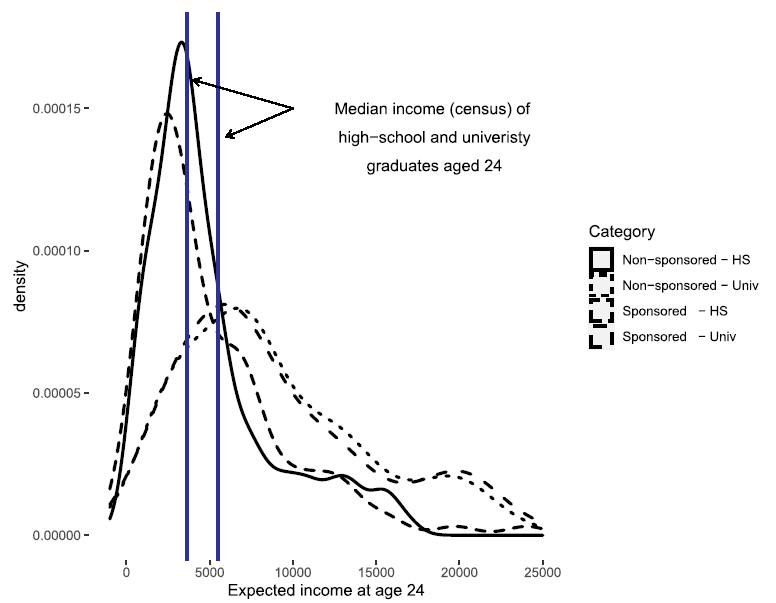
\includegraphics[width=\textwidth]{../Figures/Figure1_IncomeDist.png}
      \end{center}
    \end{column}
    \begin{column}{0.41\textwidth}
      \textbf{Reading the figure:}
      \begin{itemize}
        \item Both HS and Univ distributions are \gold{right-skewed} — consistent with log-normal income
        \item Distribution \textbf{modes} closely match census medians (vertical lines)
        \item \bad{Substantial heterogeneity}: wide right tail — some children are very optimistic
        \item Sponsored and non-sponsored distributions largely overlap
      \end{itemize}
      \begin{keybox}
        \small Children's beliefs are realistic \textit{on average} — but extremely diverse across individuals
      \end{keybox}
    \end{column}
  \end{columns}
\end{frame}

%% ============================================================
\section{Model}
%% ============================================================

%% ---- 15. Identification Challenge ---------------------------
\begin{frame}{The Core Identification Challenge}
  \begin{columns}
    \begin{column}{0.55\textwidth}
      \textbf{Naive comparison is biased:}
      \begin{itemize}
        \item Sponsored children differ from non-sponsored in observable \textit{and} unobservable ways
        \item E.g., more motivated families may seek sponsorship; CI targets the most vulnerable
        \item Raw difference in aspirations $\neq$ causal effect of CI
      \end{itemize}
      \vspace{0.5em}
      \textbf{Standard IV approach (LATE):}
      \begin{itemize}
        \item Identifies effect only for compliers
        \item Assumes $\alpha_1 = \alpha_0$ (no selection on gains)
        \item Misses heterogeneity in treatment effects
      \end{itemize}
    \end{column}
    \begin{column}{0.41\textwidth}
      \begin{methodbox}
        \textbf{This paper:} Binary Roy-type model \citep{Aakvik2005}
        \begin{itemize}
          \item Allows selection on unobserved gains ($\alpha_1 \neq \alpha_0$)
          \item Identifies ATE, ATT, \textit{and} MTE
          \item Discrete outcome is more natural for educational aspirations (target-based)
        \end{itemize}
      \end{methodbox}
    \end{column}
  \end{columns}
\end{frame}

%% ---- 16. Roy Model Overview ---------------------------------
\begin{frame}{Roy Model: Three-Equation System}
  \textbf{Three latent variable equations:}

  \vspace{0.4em}
  \textbf{1.\ Selection equation} — who gets sponsored:
  \[
    S^*_i = Z_i\gamma - U_{Si}, \qquad S_i = \mathbf{1}[S^*_i > 0]
  \]

  \textbf{2.\ Outcome for sponsored} ($S_i=1$):
  \[
    Y^*_{1i} = \beta^1_0 + \rho_{HE,i}\,\beta^1_2 + \mathit{Dist}_i\,\beta^1_3 + \tilde{X}_i\,\beta^1_4 - U_{1i}
  \]

  \textbf{3.\ Outcome for non-sponsored} ($S_i=0$):
  \[
    Y^*_{0i} = \beta^0_0 + \rho_{HE,i}\,\beta^0_2 + \mathit{Dist}_i\,\beta^0_3 + \tilde{X}_i\,\beta^0_4 - U_{0i}
  \]

  \vspace{0.3em}
  Observed outcome: $Y_i = S_i Y_{1i} + (1-S_i)Y_{0i}$, where $Y_{ji} = \mathbf{1}[Y^*_{ji}>0]$
\end{frame}

%% ---- 17. Selection Equation ---------------------------------
\begin{frame}{Selection Equation: Regressors and Exclusion Restrictions}
  \[
    S^*_i = \gamma_0 + \sum_{p=6}^{8} \mathit{Age}p_i\,\gamma_p + \mathit{AssetIndex}_i\,\gamma_4 + \mathit{Protestant}_i\,\gamma_5 + \mathit{SiteCI}_i\,\gamma_6 - U_{Si}
  \]

  \vspace{0.4em}
  \begin{columns}
    \begin{column}{0.50\textwidth}
      \textbf{Exclusion restrictions:} $\mathit{Agep}$ dummies
      \begin{itemize}
        \item $\mathit{Agep} = 1$ if child was $p$ years old when CI arrived in the village ($p \in \{6,7,8\}$)
        \item Omitted category: age 9 or older (too old to be eligible)
        \item \gold{Intuition:} younger children when CI arrived $\Rightarrow$ higher probability of being sponsored — but age-at-arrival should not directly affect current aspiration
      \end{itemize}
    \end{column}
    \begin{column}{0.46\textwidth}
      \begin{assumptionbox}[Exclusion restriction]
        $\mathit{Agep}$ affects selection probability but not aspirations directly — valid if aspirations depend on current characteristics, not age at program arrival
      \end{assumptionbox}
      \vspace{0.3em}
      \textbf{Other controls:} Asset index (wealth), Protestant (church attendance), CI site dummy
    \end{column}
  \end{columns}
\end{frame}

%% ---- 18. Outcome Equations ----------------------------------
\begin{frame}{Outcome Equations: Key Regressors}
  \begin{columns}
    \begin{column}{0.50\textwidth}
      \textbf{Regressors} $X_i = (1,\, \rho_{HE,i},\, \mathit{Dist}_i,\, \tilde{X}_i)$:
      \begin{itemize}
        \item $\rho_{HE,i}$: \gold{perceived returns to higher education} — enters as extra variable (in Model 2)
        \item $\mathit{Dist}_i$: distance to nearest university (km) — access proxy
        \item $\tilde{X}_i$: gender, asset index, parental education, Prospera dummy
      \end{itemize}
    \end{column}
    \begin{column}{0.46\textwidth}
      \textbf{Why $\rho_{HE}$ matters:}
      \begin{itemize}
        \item Tests whether \textit{subjective expectations about returns} shape aspirations
        \item \citet{Jensen2010}, \citet{Nguyen2008}: information about returns can shift schooling choices
        \item If $\beta^1_2$ or $\beta^0_2$ significant: subjective beliefs drive aspirations
        \item If not: other factors (internal constraints, income, social context) dominate
      \end{itemize}
    \end{column}
  \end{columns}
\end{frame}

%% ---- 19. Error Structure ------------------------------------
\begin{frame}{One-Factor Error Structure}
  \textbf{The error terms share a common latent factor $\theta_i$:}
  \[
    U_{Si} = -\theta_i + \varepsilon_{Si}, \qquad
    U_{1i} = -\alpha_1\theta_i + \varepsilon_{1i}, \qquad
    U_{0i} = -\alpha_0\theta_i + \varepsilon_{0i}
  \]

  \vspace{0.3em}
  \begin{columns}
    \begin{column}{0.55\textwidth}
      \textbf{What this allows:}
      \begin{itemize}
        \item Non-zero correlation between $U_{Si}$ and $U_{ji}$: $\mathrm{Cov}(U_S, U_1) = \alpha_1$, $\mathrm{Cov}(U_S, U_0) = \alpha_0$
        \item Selection on \textit{unobserved gains}: $\alpha_1 \neq \alpha_0$
        \item Recovers joint distribution of $(U_S, U_1, U_0)$ under normality
      \end{itemize}
      \vspace{0.3em}
      Normalization: $\mathrm{Var}(\theta_i) = \mathrm{Var}(\varepsilon_{ji}) = 1\;\forall i$
    \end{column}
    \begin{column}{0.41\textwidth}
      \begin{methodbox}
        \small \textbf{vs.\ IV:} IV assumes $\alpha_1 = \alpha_0$ (no selection on gains). The Roy model relaxes this. More flexible, but requires the normality assumption.
      \end{methodbox}
    \end{column}
  \end{columns}
\end{frame}

%% ---- 20. MLE Estimation -------------------------------------
\begin{frame}{Estimation: Maximum Likelihood}
  Integrate over the unobserved factor $\theta_i$:
  \[
    L = \prod_{i=1}^{N} \int \Pr(S_i, Y_i \mid X_i, Z_i, \theta_i)\, \phi(\theta_i)\, d\theta_i
  \]

  where:
  \begin{align*}
    \Pr(Y_i=1 \mid S_i=1, X_i, \theta_i) &= \Phi(X_i\hat{\beta}_1 + \hat{\alpha}_1\theta_i) \\
    \Pr(Y_i=1 \mid S_i=0, X_i, \theta_i) &= \Phi(X_i\hat{\beta}_0 + \hat{\alpha}_0\theta_i) \\
    \Pr(S_i=1 \mid Z_i, \theta_i) &= \Phi(Z_i\hat{\gamma} + \theta_i)
  \end{align*}

  \vspace{0.3em}
  \begin{methodbox}
    \textbf{Numerical integration:} Gauss-Hermite quadrature with 10 nodes — accurate approximation to the normal integral over $\theta_i$. Standard errors via bootstrapping.
  \end{methodbox}
\end{frame}

%% ---- 21. Treatment Effects ----------------------------------
\begin{frame}{Treatment Effects: ATE, ATT, MTE}
  \begin{columns}
    \begin{column}{0.48\textwidth}
      \textbf{Average Treatment Effect (ATE):}
      \[
        \ATE(x) = \Phi\!\left(\frac{x\hat{\beta}_1}{\sqrt{1+\hat{\alpha}_1^2}}\right) - \Phi\!\left(\frac{x\hat{\beta}_0}{\sqrt{1+\hat{\alpha}_0^2}}\right)
      \]
      Average over all children with characteristics $x$

      \vspace{0.6em}
      \textbf{Average Treatment on Treated (ATT):}
      \[
        \ATT(x, S=1) = \frac{1}{F_{U_S}(z\hat{\gamma})} \left[F_{U_S, U_1}(\cdot) - F_{U_S, U_0}(\cdot)\right]
      \]
      Average only over sponsored children
    \end{column}
    \begin{column}{0.48\textwidth}
      \textbf{Marginal Treatment Effect (MTE):}
      \[
        \MTE(x, u_S) = \Pr(Y_1=1 \mid X=x, U_S=u_S) - \Pr(Y_0=1 \mid X=x, U_S=u_S)
      \]
      Effect for children at the \gold{margin of selection} $u_S$

      \vspace{0.4em}
      \begin{keybox}
        \small MTE is a \textbf{building block}: ATE and ATT are weighted averages of MTE with appropriate weights \citep{Heckman2007}
      \end{keybox}
    \end{column}
  \end{columns}
\end{frame}

%% ============================================================
\section{Results}
%% ============================================================

%% ---- 22. Selection Equation Results -------------------------
\begin{frame}{Selection Results: Who Gets Sponsored?}
  \textbf{Table 3: Selection equation (Model 1, N=403)}
  \begin{center}
  \begin{tabular}{lcccc}
    \toprule
    & \multicolumn{2}{c}{\textbf{Model 1}} & \multicolumn{2}{c}{\textbf{Model 2}} \\
    & Coeff. & Marg. effect & Coeff. & Marg. effect \\
    \midrule
    Dummy(Age 6) & 1.19*** & 0.215*** & 1.69*** & 0.257*** \\
    Dummy(Age 7) & 1.63*** & 0.210*** & 1.85*** & 0.285*** \\
    Dummy(Age 8) & 1.43*** & 0.259*** & 1.67*** & 0.271*** \\
    Protestant    & 1.31*** & 0.236*** & 1.92*** & 0.338*** \\
    Asset index   & $-$0.165** & $-$0.029** & $-$0.27*** & $-$0.043*** \\
    Treated site  & 3.313 & 0.599*** & 3.149 & 0.432*** \\
    \bottomrule
  \end{tabular}
  \end{center}
  \vspace{0.3em}
  \begin{itemize}
    \item \gold{Younger cohorts} at arrival: $\approx$21--26 pp more likely to be selected (\textit{exclusion restriction works})
    \item \gold{Protestant}: $\approx$24--34 pp more likely (church affiliation, not religiosity)
    \item \bad{Higher asset index}: $\approx$3--4 pp less likely — CI targets poorer households
  \end{itemize}
\end{frame}

%% ---- 23. Outcome Equation Results ---------------------------
\begin{frame}{Outcome Results: What Drives Aspirations? (Model 1)}
  \textbf{Table 4: Marginal effects (Model 1, N=403). Standard errors in parentheses.}
  \begin{center}
  \small
  \begin{tabular}{lcc}
    \toprule
    & \textbf{Sponsored} & \textbf{Non-Sponsored} \\
    \midrule
    Dummy(Prospera)            & 0.057 (0.108)   & 0.076 (0.091)    \\
    Dummy(Male)                & $-$0.043 (0.074)  & $-$0.119** (0.055) \\
    Asset Index                & 0.016 (0.024)   & 0.336*** (0.022) \\
    Parental Education         & 0.027** (0.013) & 0.023** (0.010)  \\
    Distance to Univ.\ (km)   & $-$0.006 (0.0008) & 0.0004 (0.0008)  \\
    \midrule
    $E[\ATE(x)]$               & \multicolumn{2}{c}{0.016 \quad (0.083)} \\
    $E[\ATT(x)]$               & \multicolumn{2}{c}{0.170 \quad (0.183)} \\
    \bottomrule
  \end{tabular}
  \end{center}
  \vspace{0.2em}
  \begin{small}*** $p{<}0.01$, ** $p{<}0.05$, * $p{<}0.1$. Bootstrap standard errors.\end{small}
\end{frame}

%% ---- 23b. Outcome Equation Results Model 2 -----------------
\begin{frame}{Outcome Results: Model 2 (Adding Subjective Expectations)}
  \textbf{Table 4: Marginal effects (Model 2, N=271). Standard errors in parentheses.}
  \begin{center}
  \small
  \begin{tabular}{lcc}
    \toprule
    & \textbf{Sponsored} & \textbf{Non-Sponsored} \\
    \midrule
    Dummy(Prospera)            & 0.112 (0.154)     & 0.005 (0.127)    \\
    Dummy(Male)                & $-$0.078 (0.097)  & $-$0.035 (0.08)  \\
    Asset Index                & $-$0.011 (0.033)  & 0.06** (0.03)    \\
    Parental Education         & 0.05*** (0.017)   & 0.024 (0.015)    \\
    Distance to Univ.\ (km)   & 0.000 (0.001)     & 0.001 (0.001)    \\
    $\rho_{HE}$                & $-$0.113 (0.072)  & 0.016 (0.069)    \\
    \midrule
    $E[\ATE(x)]$               & \multicolumn{2}{c}{$-$0.008 \quad (0.009)} \\
    $E[\ATT(x)]$               & \multicolumn{2}{c}{0.204 \quad (0.180)} \\
    \bottomrule
  \end{tabular}
  \end{center}
  \vspace{0.1em}
  \begin{small}*** $p{<}0.01$, ** $p{<}0.05$, * $p{<}0.1$. Bootstrap SEs. Restricted to children who correctly interpreted probability questions.\end{small}
\end{frame}

%% ---- 24. Mean Sponsorship Effects ---------------------------
\begin{frame}{Mean Sponsorship Effects: Positive but Imprecise}
  \begin{columns}
    \begin{column}{0.55\textwidth}
      \textbf{Average treatment effect on the treated (ATT):}
      \begin{itemize}
        \item Model 1: CI's estimated ATT $\approx$ \gold{17 percentage points} increase in aspiration probability
        \item Model 2 (with $\rho_{HE}$): $\approx$ \gold{20 percentage points}
        \item Direction consistent with prior CI studies
        \item \bad{Not statistically significant} — large standard errors due to small sample + bootstrap
      \end{itemize}
      \vspace{0.5em}
      \textbf{How to interpret imprecision:}
      \begin{itemize}
        \item Coefficients estimated via MLE with integration — inherently noisier than OLS
        \item Results should be read as \textit{suggestive} evidence, not definitive
      \end{itemize}
    \end{column}
    \begin{column}{0.41\textwidth}
      \begin{resultbox}
        \textbf{Back-of-envelope:} If aspirations translate to behavior, a 20 pp increase in aspiration implies $\approx$ \textbf{8 more months of schooling} — consistent with \citet{Wydick2013} who find 1.03--1.46 additional years for adult outcomes
      \end{resultbox}
    \end{column}
  \end{columns}
\end{frame}

%% ---- 25. Why Not Significant? -------------------------------
\begin{frame}{Why Not Statistically Significant?}
  \begin{columns}
    \begin{column}{0.55\textwidth}
      \textbf{Statistical explanation:}
      \begin{itemize}
        \item Small sample ($N=163$ sponsored)
        \item MLE with integration amplifies standard errors
        \item Binary Roy model has many parameters
        \item Bootstrapped SEs inflate uncertainty further
      \end{itemize}
      \vspace{0.5em}
      \textbf{Substantive interpretation:}
      \begin{itemize}
        \item Aspirations at ages 12--15 may be driven by factors CI doesn't directly address: self-esteem, optimism (Ross et al., 2021 found no CI effect on self-esteem in Mexico)
        \item In rural contexts, aspiring to higher education may be perceived as \textit{unrealistically ambitious}
        \item Short-term attainable goals may matter more at this stage \citep{Genicot2017}
      \end{itemize}
    \end{column}
    \begin{column}{0.41\textwidth}
      \begin{keybox}
        \textbf{Proposed mechanism} (to explain the positive effect found in the literature): Anecdotal evidence and local CI staff report that school attendance is \textit{de facto} required for continued sponsorship\\[0.5em]
        $\Rightarrow$ More time in school $\Rightarrow$ stronger educational identity
      \end{keybox}
    \end{column}
  \end{columns}
\end{frame}

%% ---- 26. MTE Figure -----------------------------------------
\begin{frame}{Marginal Treatment Effect: Targeting Efficiency}
  \begin{columns}
    \begin{column}{0.55\textwidth}
      \begin{center}
        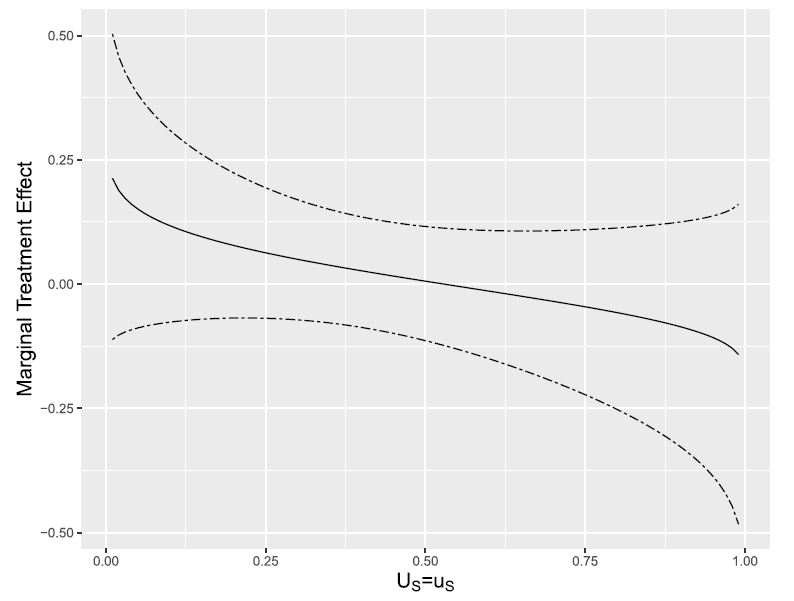
\includegraphics[width=\textwidth]{../Figures/Figure2_MTE.png}
      \end{center}
    \end{column}
    \begin{column}{0.41\textwidth}
      \textbf{Reading the MTE curve:}
      \begin{itemize}
        \item $u_S$ = unobserved resistance to selection
        \item Low $u_S$: children \gold{most likely} to be selected into CI
        \item High $u_S$: children \gold{least likely} to be selected
      \end{itemize}
      \vspace{0.3em}
      \textbf{Pattern:} MTE declines in $u_S$
      \begin{itemize}
        \item Sponsored children exhibit \textit{higher} sponsorship effect
        \item Positive correlation between selection and treatment effect
      \end{itemize}
    \end{column}
  \end{columns}
\end{frame}

%% ---- 27. MTE Interpretation ---------------------------------
\begin{frame}{MTE Interpretation: No Efficiency-Equity Trade-Off}
  \begin{columns}
    \begin{column}{0.55\textwidth}
      \textbf{Key finding from MTE:}
      \[
        \mathrm{Cov}(U_S, U_1) = \alpha_1 > 0
      \]
      Children who are \gold{more likely to be selected} are also those who \gold{benefit more} from sponsorship

      \vspace{0.5em}
      \textbf{Policy implication for CI:}
      \begin{itemize}
        \item Aid agencies often face efficiency vs.\ equity trade-off: targeting most-vulnerable $\neq$ targeting those with highest gains
        \item \pos{CI does not face this trade-off} in this context: the most vulnerable also benefit the most
        \item Reassuring for CI's targeting strategy
      \end{itemize}
    \end{column}
    \begin{column}{0.41\textwidth}
      \begin{resultbox}
        \textbf{Formal result:} The positive correlation between selection propensity and treatment effect means CI's self-selected targeting is \textit{efficient} — children most in need extract the greatest gains
      \end{resultbox}
    \end{column}
  \end{columns}
\end{frame}

%% ---- 28. Subjective Beliefs & Aspirations -------------------
\begin{frame}{Do Subjective Income Beliefs Drive Aspirations?}
  \begin{columns}
    \begin{column}{0.55\textwidth}
      \textbf{Result:} $\rho_{HE}$ (perceived returns to higher education) is \bad{not statistically significant} in either the sponsored or non-sponsored outcome equations (Model 2)

      \vspace{0.5em}
      \textbf{Two possible interpretations:}
      \begin{enumerate}
        \item Children age 12--15 are too young to integrate income beliefs into long-run plans — other factors dominate (external constraints, identity, social context)
        \item Low levels of education in rural communities make higher education \textit{aspirationally unrealistic}, even with accurate income beliefs
      \end{enumerate}
    \end{column}
    \begin{column}{0.41\textwidth}
      \begin{keybox}
        \small Related to \citet{Genicot2017}: \textit{feasibility} matters as much as desirability. If a goal is perceived as unattainable, even high expected returns won't shift aspirations.\\[0.5em]
        $\Rightarrow$ Short-term attainable milestones may be more effective than long-run income arguments
      \end{keybox}
    \end{column}
  \end{columns}
\end{frame}

%% ---- 29. Gender Gap -----------------------------------------
\begin{frame}{Gender Gap in Aspirations and Income Expectations}
  \begin{columns}
    \begin{column}{0.55\textwidth}
      \textbf{Aspirations (outcome equation):}
      \begin{itemize}
        \item Being male $\Rightarrow$ \bad{lower} aspiration for higher education
        \item Non-sponsored: marginal effect of being male $\approx -0.12$ (significant)
        \item Sponsored: same sign, not significant
      \end{itemize}

      \vspace{0.5em}
      \textbf{Income expectations (Table 2):}
      \begin{itemize}
        \item Females expect $\approx$\bad{50\% lower income} than males at high-school level
        \item Gender gap exists even among 12--15 year olds
        \item Females have \textit{higher} aspirations despite expecting \textit{lower} income — gap is \gold{not explained by income beliefs}
      \end{itemize}
    \end{column}
    \begin{column}{0.41\textwidth}
      \begin{resultbox}
        \textbf{Puzzle:} Females aspire more to higher education than males — yet expect substantially lower earnings. Suggests aspirations and income expectations are driven by \textit{different} mechanisms for boys and girls
      \end{resultbox}
    \end{column}
  \end{columns}
\end{frame}

%% ============================================================
\section{Discussion \& Conclusions}
%% ============================================================

%% ---- 30. Discussion -----------------------------------------
\begin{frame}{Discussion: Mechanisms}
  \textbf{Why does CI have a positive (if imprecise) effect on aspirations?}
  \begin{itemize}
    \item \gold{School attendance mechanism}: CI de facto requires attendance as condition for continued support $\Rightarrow$ more time in school $\Rightarrow$ stronger educational identity
    \item \gold{Horizon broadening}: letter exchanges with international sponsors expose children to different careers and life outcomes
    \item Not via self-esteem or optimism \citep{Ross2021} — and not via income beliefs (this paper)
  \end{itemize}
\end{frame}

%% ---- 31. Robustness Checks ----------------------------------
\begin{frame}{Robustness}
  \textbf{Main results are robust to:}

  \begin{enumerate}
    \item \textbf{Distributional assumption for income}: Uniform distribution (instead of triangular) for $f(Y^\ell)$ — nearly identical estimates
    \item \textbf{Prospera overlap}: $\approx$85\% of sample participates in Prospera (conditional cash transfer). Assuming Prospera affects both groups equally and re-estimating on Prospera participants only: conclusions unchanged
    \item \textbf{Standard Roy model with continuous outcome + IV}: Using exclusion restrictions as instruments; results not statistically significant either (Table 9, Appendix)
    \item \textbf{Alternative controls}: Removing asset index, distance, or location variables; main conclusions unchanged (Table 11, Appendix)
  \end{enumerate}

  \vspace{0.3em}
  \begin{keybox}
    The direction of the effect (positive ATT) and the non-significance are robust across all specifications
  \end{keybox}
\end{frame}

%% ---- 32. Conclusions ----------------------------------------
\begin{frame}{Conclusions}
  \begin{enumerate}
    \item \navy{CI has a positive effect on aspirations} among rural Mexican children (ages 12--15) — estimated ATT of 17--20 pp — but \bad{not statistically significant}
    \begin{itemize}
      \item Results should be read as suggestive; consistent with prior CI evidence on adult outcomes
    \end{itemize}

    \item \navy{CI's targeting is efficient:} the children most likely to be selected are also those who benefit most — no efficiency-equity trade-off

    \item \navy{Subjective income beliefs do not significantly predict aspirations} at ages 12--15 in this rural context — other factors dominate

    \item \navy{Clear gender gap:} females aspire more to higher education than males, yet expect substantially lower future earnings — the gap is not driven by income beliefs

    \item \navy{Methodological contribution:} applying the binary Roy model to a child sponsorship program enables a richer characterization of treatment effect heterogeneity than IV or standard probit approaches
  \end{enumerate}
\end{frame}

%% ---- 33. Policy Implications --------------------------------
\begin{frame}{Policy Implications}
  \begin{columns}
    \begin{column}{0.50\textwidth}
      \textbf{For child sponsorship programs:}
      \begin{itemize}
        \item Holistic programs that \gold{combine material support with socio-emotional development} appear well-positioned to shift aspirations
        \item Emphasize \gold{short-term attainable goals} alongside long-run aspirations — realistic milestones may be more actionable than abstract future income
        \item School attendance requirements (even informal) may be a valuable design feature
      \end{itemize}
    \end{column}
    \begin{column}{0.46\textwidth}
      \textbf{For gender equity:}
      \begin{itemize}
        \item Gender gap in income expectations starts early (ages 12--15)
        \item Information interventions about female returns may be insufficient — structural constraints and identity formation play a larger role at this age
        \item Programs should address gender-specific barriers explicitly
      \end{itemize}
      \begin{keybox}
        \small Intervening early (ages 9--12) may be more productive than waiting for aspirations to be fully formed
      \end{keybox}
    \end{column}
  \end{columns}
\end{frame}

%% ---- Bibliography -------------------------------------------
\begin{frame}[allowframebreaks]{References}
  \tiny
  \bibliography{../Bibliography_base}
\end{frame}

%% [APPENDIX COMMENTED OUT -- uncomment lines 853-935 to restore]
% %% ============================================================
% %% APPENDIX
% %% ============================================================
% \appendix
% 
% \begin{frame}[plain]
%   \begin{tikzpicture}[remember picture, overlay]
%     \fill[navyblue] (current page.south west) rectangle (current page.north east);
%     \node[white, font=\bfseries\LARGE] at (current page.center) {Appendix};
%   \end{tikzpicture}
% \end{frame}
% 
% %% ---- A1. Detailed Summary Stats -----------------------------
% \begin{frame}{A1: Summary Statistics by Group (Tables 6 \& 7)}
%   \begin{itemize}
%     \item Tables 6 and 7 present summary statistics stratified by:
%     \begin{enumerate}
%       \item Sponsored vs.\ non-sponsored siblings of sponsored children
%       \item Non-sponsored in CI communities vs.\ households in communities without CI
%     \end{enumerate}
%     \item Results remain consistent: no statistically significant differences in most demographic variables across groups
%     \item Asset index differences persist and are consistent with CI's targeting criteria
%     \item Table 8 provides a community-level comparison: CI and non-CI communities are comparable on observable characteristics at the community level
%   \end{itemize}
% \end{frame}
% 
% %% ---- A2. Figure 3: Gender Income Distribution ---------------
% \begin{frame}{A2: Income Distribution by Gender}
%   \begin{center}
%     \fbox{\parbox{0.85\textwidth}{\centering\vspace{3em}
%       \textit{Figure 3 from paper (Appendix):}\\
%       Distribution of expected income\\
%       by gender and education level\\
%       \vspace{3em}}}
%   \end{center}
%   \begin{small}
%     The figure illustrates the gender gap in income expectations more clearly: male distribution is shifted right relative to female distribution, especially at the high-school level. The gap is smaller at the university level, consistent with Table 2.
%   \end{small}
% \end{frame}
% 
% %% ---- A3. Robustness: Standard Roy + IV ----------------------
% \begin{frame}{A3: Robustness — Standard Roy Model and IV (Table 9)}
%   \textbf{Two additional specifications:}
%   \begin{columns}
%     \begin{column}{0.48\textwidth}
%       \textbf{Standard Roy with continuous outcome:}
%       \begin{itemize}
%         \item Treat aspiration as continuous (years of desired schooling)
%         \item Use age-at-arrival dummies as instruments
%         \item Results: CI effect \bad{not statistically significant}
%         \item Direction: positive
%         \item Consistent with main results
%       \end{itemize}
%     \end{column}
%     \begin{column}{0.48\textwidth}
%       \textbf{IV approach:}
%       \begin{itemize}
%         \item LATE identified using age-at-arrival dummies
%         \item Identifies effect only for compliers (children who would be sponsored if younger at arrival)
%         \item Results: also \bad{not significant}
%         \item Confirms that lack of significance is not an artifact of the Roy model framework
%       \end{itemize}
%     \end{column}
%   \end{columns}
% \end{frame}
% 
% %% ---- A4. MTE Estimation Steps -------------------------------
% \begin{frame}{A4: MTE Estimation Procedure (Appendix 7.3)}
%   \textbf{Step-by-step:}
%   \begin{enumerate}
%     \item Estimate parameters $(\hat{\gamma}, \hat{\alpha}_0, \hat{\alpha}_1, \hat{\beta}_0, \hat{\beta}_1)$ via MLE
%     \item Compute $U_{Si}$ quantiles from the selection equation: $\hat{u}_{Si} = \Phi(-Z_i\hat{\gamma})$ (propensity score residuals)
%     \item For a grid of $u_S$ values:
%     \[
%       \widehat{\MTE}(x, u_S) = \frac{\int [\Phi(x\hat{\beta}_1 + \hat{\alpha}_1\theta) - \Phi(x\hat{\beta}_0 + \hat{\alpha}_0\theta)]\,\phi(u_S + \theta)\,\phi(\theta)\,d\theta}{\phi(u_S)/\sqrt{2}}
%     \]
%     \item Plot MTE as function of $u_S$; bootstrap for confidence intervals
%   \end{enumerate}
%   \vspace{0.3em}
%   \begin{methodbox}
%     \small ATE and ATT are then recovered as weighted averages of MTE, using the marginal distribution of $U_S$ and $\Pr(S=1 \mid X, Z)$ as weights respectively
%   \end{methodbox}
% \end{frame}

\end{document}
